%---------------------------------------------------------------------------%
%---------------------------------------------------------------------------%
%                          MPT THEME - EXAMPLE                              %
%---------------------------------------------------------------------------%
%---------------------------------------------------------------------------%

%---------------------------------------------------------------------------%
% HEADER                                                                    %
%---------------------------------------------------------------------------%

%----- DOCUMENT TYPE--------------------------------------------------------%
%---------------------------------------------------------------------------%

\pdfminorversion = 5
\documentclass[10pt]{beamer}
\usetheme[francais %[For documents written in french]
%,notocfoot %[To remove the presentation title in the footer of the frames]
%,arial %[To use arial as the default text font instead of Linux Biolinum]
,alertred %[For the alterted text to be framed in red instead of blue]
%,euler %[To use euler as the default math font instead of XITS]
%,sober %[To remove the grey areas behind the frame titles and the footer]
]{MPTM} %[Comment and uncomment options as desired]


%----- PACKAGES-------------------------------------------------------------%
%---------------------------------------------------------------------------%
% [Put all desired packages here]

%Notes
\usepackage{pdfpages}
%\setbeameroption{show notes} %[to show note on the pdf]
%\setbeameroption{show notes on second screen=right}%Pour placer les notes à droite, en extension d'une slide mais commande qui ne marche pas


%TIKZ
\usepackage{pgfplots}

\pgfplotsset{compat=1.14}

\usetikzlibrary{calc, 3d, positioning, intersections, backgrounds, shapes, math, shapes.geometric, topaths, decorations.markings, pgfplots.colormaps}
\usepgfplotslibrary{colormaps, fillbetween}
\pgfplotsset{probastyle/.style={smooth, width = \textwidth, axis x line = bottom, axis y line = left,
		every axis x label/.style={ at={(ticklabel* cs:1.05)}, anchor=west,},
		every axis y label/.style={	at={(ticklabel* cs:1.05)}, anchor=south,}}}
\pgfplotsset{ colormap={MPT}{rgb255(0cm)=(0,94,158) rgb255(0.25cm)=(0,111,182) rgb255(1cm)=(240,240,240) rgb255(2cm)=(156,158,159)}}
\pgfplotsset{compat=newest}
\pgfplotsset{school/.style={tick align = outside, major tick length = 2.5pt, axis line style={-stealth}, anchor = center, x label style = {anchor = west, at = {(current axis.right of origin)}}, y label style = {anchor = south, at = {(current axis.above origin)}, rotate = -90}}}
\usepackage{tikz-3dplot}
\tdplotsetmaincoords{60}{-30}
\tdplotsetrotatedcoords{0}{90}{90}
\pgfmathdeclarefunction{gaussShape}{2}{%
  \pgfmathparse{(1/#2)*exp(-((x-#1)^2)/(1^2))}%
  }
  \pgfmathdeclarefunction{gauss}{2}{%
  \pgfmathparse{(1/(#2*sqrt(2*pi)))*exp(-((x-#1)^2)/(2*#2^2))}%
}
\tikzset{
		    base/.style = {draw=MPTgrey, ultra thick, 
			minimum height=30mm, minimum width=30mm,
			inner sep=0pt}, %permet d'afficher une image dans un rectangle
  invisible/.style={opacity=0},
  visible on/.style={alt={#1{}{invisible}}},
  alt/.code args={<#1>#2#3}{%
    \alt<#1>{\pgfkeysalso{#2}}{\pgfkeysalso{#3}} % \pgfkeysalso doesn't change the path
  },
}
\usetikzlibrary{arrows.meta}

%smiley souriant bleu
\newcommand{\smiley}{\tikz[baseline=-0.75ex,black]{
		\draw[MPTblue] circle (2mm);
		\node[MPTblue,fill,circle,inner sep=0.5pt] (left eye) at (135:0.8mm) {};
		\node[MPTblue,fill,circle,inner sep=0.5pt] (right eye) at (45:0.8mm) {};
		\draw[MPTblue] (-145:0.9mm) arc (-120:-60:1.5mm);
	}
}

%smiley pas content rouge
\newcommand{\frownie}{\tikz[baseline=-0.75ex,black]{
		\draw[MPTred] circle (2mm);
		\node[MPTred,fill,circle,inner sep=0.5pt] (left eye) at (135:0.8mm) {};
		\node[MPTred,fill,circle,inner sep=0.5pt] (right eye) at (45:0.8mm) {};
		\draw[MPTred](-145:0.9mm) arc (120:60:1.5mm);
	}
}


%----- MATH
%\usepackage{amsmath, amssymb, amscd, latexsym, bigints, stmaryrd, bm}
\usepackage{stmaryrd, bm}

%----- TABLES
\usepackage{booktabs, tabularx, multirow, colortbl}
\arrayrulecolor{main}
\setlength{\aboverulesep}{0pt}
\setlength{\belowrulesep}{0pt}
\setlength{\extrarowheight}{5pt}
\newcolumntype{L}{>{\raggedright\arraybackslash}X}
\newcolumntype{R}{>{\raggedleft\arraybackslash}X}
\newcolumntype{C}{>{\centering\arraybackslash}X}
\newcolumntype{s}{@{\hspace{3pt}} c @{\hspace{6pt}}}

%----- FIGURES
\usepackage{graphicx, psfrag, color, epsfig}   % to include and manipulate graphics
\usepackage[all]{xy}    % to draw diagrams
%\usepackage{ifsym}
\usepackage{multirow}

%----- LISTS
\usepackage{enumerate}

%----- BIBLIO
\usepackage{bibentry}

%-----BARRER
\usepackage{soul}

%----- SYMBOLS
\usepackage{pifont}
\usepackage{bclogo}

%----Font
\usepackage{verbatim}
\usepackage{fancyvrb}
\makeatletter
\newcommand{\verbatimfont}[1]{\renewcommand{\verbatim@font}{\ttfamily#1}}
\makeatother

%\usepackage{secdot}
%\sectiondot{subsection}

%----- ADDITIONAL COMMANDS 
%---------------------------------------------------------------------------
\newcommand{\bfun}{\bm{1}}
%\let\sectionOld\section
%\renewcommand\section[2][\empty]{%boldmath\sectionOld[#1]{#2}\unboldmath%}
% [Put all user-defined commands here]

%----- Symbols
\newcommand{\ex}{{\color{MPTblue}\ding{228}}}
%\newcommand{\ex}{{\color{MPTblue}\small{\blacktriangleright}}}

%----- SPACES
\newcommand{\hsp}{\hspace*{1em}}
\newcommand{\midhsp}{\hspace*{.5em}}

\makeatletter
\define@key{beamerframe}{c}[true]{% centered
	\beamer@frametopskip=0pt plus 1fill\relax%
	\beamer@framebottomskip=0pt plus 1fill\relax%
	\beamer@frametopskipautobreak=0pt plus .4\paperheight\relax%
	\beamer@framebottomskipautobreak=0pt plus .6\paperheight\relax%
	\def\beamer@initfirstlineunskip{}%
}
\makeatother

%Version étudiants
\usepackage{ifthen}
\newboolean{showToPublic}
\setboolean{showToPublic}{true}
%\newcommand{\todocmd}[2]{{{#1}}{{#2}}}
\newcommand{\todo}[2]{\ifthenelse {\boolean{showToPublic}}{#1}{#2}} %{\todocmd{#1}}{\todocmd{#2}}}




%----- BIBLIO
\newcommand{\itbib}[1]{{\itshape \bibentry{#1}}}
%\providecommand{\bysame}{S.I. Resnick}%

%----- PATHS
%---------------------------------------------------------------------------%
\graphicspath{{Images/}}	%[Indicate the name of the file where your images are stored]

%---------------------------------------------------------------------------%
% TITLE                                                                     %
%---------------------------------------------------------------------------%

\title{Apprentissage supervisé et non supervisé}
\subtitle{
	{}}
\author{}
%\institute{Mines ParisTech}{Equipe Géostatistique}{}
%\coauthor{Sophie Lèbre}
%\coauthor[2]{Anne Sabourin}
%\coinstitute{Mines ParisTech}{Equipe Géostatistique}{}
%\coinstitute[2]{Telecom Paris}{Equipe S2A}{}
\date{}
\event{M1 MIASHS}
%\subtitle{Subtitle}
\rclogo{}	% Research center(s) logo(s)
\netlogo{}	% Partner(s)  logo(s) separated by comma




%---------------------------------------------------------------------------%
% PRESENTATION                                                              %
%---------------------------------------------------------------------------%
\begin{document}
	
%---------------------------------------------------------------------------%
% TITLE FRAME                                                               %
%---------------------------------------------------------------------------%
\begin{frame}
	\maketitle
\end{frame}

%---------------------------------------------------------------------------%
% TOC SETUP                                                                 %
%---------------------------------------------------------------------------%

%Ce qui est affiché quand on a la commande \section{}

\AtBeginSection[]{
	{
		\usebackgroundtemplate{
			\begin{tikzpicture} [inner sep = 0pt, outer sep = 0pt]
			
			%----- MASK - \pgflinewidth
			\node [anchor = north west, minimum width = \paperwidth - \pgflinewidth, minimum height = \paperheight - \pgflinewidth] (pc) at (current page.north west) {};
			
			%----- BACKGROUND
			\shade[top color = event.bg, bottom color = white] (pc.north west) rectangle ([yshift = -15pt]pc.north east);
			\shade[bottom color = event.bg, top color = white] (pc.south west) rectangle ([yshift = 15pt]pc.south east);
			
			----- SECTION NUMBER %[Uncomment if you want the section number to appear in the background]
			\node[minimum height = .9\paperheight, anchor = center] at (current page.center) 				 {\color{event.bg}{\fontsize{300}{0}\selectfont \Roman{section}}};
			
			%----- TITLE SECTION
			\node[anchor = center, text centered] at (current page.center) {\begin{minipage}[c]{.9\textwidth} \centering \huge\bfseries\scshape\color{MPTblue}\insertsection
			\end{minipage}};
			
			%%----- BACK/PROB/STAT/ALGO %pour rajouter des logos sur la page de section
			%\node[anchor = north west] at ([xshift = 1em, yshift = -2em]current page.north west) {
%				\ifnumequal{\value{section}}{1}{
\includegraphics[width = 2cm]{Back.pdf}}{}
			%};
			\end{tikzpicture}
		}
		\begin{frame}[noframenumbering, plain]
			
		\end{frame}
	}
}


%Ce qui est affiché quand on a la commande \subsection{}
\AtBeginSubsection[]{
	{
		\usebackgroundtemplate{
			\begin{tikzpicture} [inner sep = 0pt, outer sep = 0pt]
				
				%----- MASK - \pgflinewidth
				\node [anchor = north west, minimum width = \paperwidth - \pgflinewidth, minimum height = \paperheight - \pgflinewidth] (pc) at (current page.north west) {};
				
				%----- BACKGROUND
				\shade[top color = event.bg, bottom color = white] (pc.north west) rectangle ([yshift = -15pt]pc.north east);
				\shade[bottom color = event.bg, top color = white] (pc.south west) rectangle ([yshift = 15pt]pc.south east);
				
				----- SECTION NUMBER %[Uncomment if you want the section number to appear in the background]
				\node[minimum height = .9\paperheight, anchor = center] at (current page.center)
				{\color{event.bg}{\fontsize{300}{0}\selectfont\Roman{section}}};

			
			%----- TITLE SUBSECTION
			\node[anchor = center, text centered] (sub) at (
			%[yshift = - \insep-1.8cm]
			current page.center) {\begin{minipage}[c]{.9\textwidth} \centering
			\LARGE\bfseries\scshape\color{MPTgrey}\Alph{subsection}.
			\insertsubsection
			\end{minipage}};
		\node[text centered] at ([yshift =  50]sub.north) {\begin{minipage}[c]{.9\textwidth} \centering
				\huge\bfseries\scshape\color{MPTblue}\insertsection
		\end{minipage}};
							\end{tikzpicture}
		}
		\begin{frame}[noframenumbering, plain]
			
		\end{frame}
	}
}

%Ce qui est affiché quand on a la commande \subsubsection{}
\AtBeginSubsubsection[]{
	{
		\usebackgroundtemplate{
			\begin{tikzpicture} [inner sep = 0pt, outer sep = 0pt]
				
				%----- MASK - \pgflinewidth
				\node [anchor = north west, minimum width = \paperwidth - \pgflinewidth, minimum height = \paperheight - \pgflinewidth] (pc) at (current page.north west) {};
				
				%----- BACKGROUND
				\shade[top color = event.bg, bottom color = white] (pc.north west) rectangle ([yshift = -15pt]pc.north east);
				\shade[bottom color = event.bg, top color = white] (pc.south west) rectangle ([yshift = 15pt]pc.south east);
				
				----- SECTION NUMBER %[Uncomment if you want the section number to appear in the background]
				\node[minimum height = .9\paperheight, anchor = center] at (current page.center)
				{\color{event.bg}{\fontsize{300}{0}\selectfont\Roman{section}}};
				
				
				%----- TITLE SUBSECTION
				\node[anchor = center, text centered] (subsub) at (
				%[yshift = - \insep-1.8cm]
				current page.center) {\begin{minipage}[c]{.9\textwidth} \centering \Large\bfseries\scshape\color{black!70!white}\arabic{subsubsection}. 
						\insertsubsubsection
				\end{minipage}};
						\node[text centered] (sub) at ([yshift =  40]subsub.north) {\begin{minipage}[c]{.9\textwidth} \centering
					\LARGE\bfseries\scshape\color{MPTgrey}\Alph{subsection}.
					\insertsubsection
			\end{minipage}};
			\node[text centered] at ([yshift =  30]sub.north) {\begin{minipage}[c]{.9\textwidth} \centering
					\huge\bfseries\scshape\color{MPTblue}\insertsection
			\end{minipage}};
			\end{tikzpicture}
		}
		\begin{frame}[noframenumbering, plain]
			
		\end{frame}
	}
}




%---------------------------------------------------------------------------%
% INTRODUCTION                                                              %
%---------------------------------------------------------------------------%
%
%---------------------------------------------------------------------------%
%
%
%---------------------------------------------------------------------------%
%


%\begin{frame}[fragile, noframenumbering]
%	\bftitle{Intervenantes}\hspace{1.7em}  Sophie Lèbre, Marine Demangeot\\[3em]
%	\bftitle{5 cours} \hspace{5em} mercredi 21 septembre \hspace{0.3em} \textcolor{MPTgrey}{(9h00-12h15)} \hfill \\[0.2em]
%	\phantom{\bftitle{5 cours} }  \hspace{5em} jeudi 22 septembre \hspace{1.6em} \textcolor{MPTgrey}{(9h00-12h15)} \hfill \\[0.2em]
%	\phantom{\bftitle{5 cours} }  \hspace{5em} lundi 10 octobre \hspace{2.8em} \textcolor{MPTgrey}{(9h00-12h15)} \hfill \\[0.2em]
%	\phantom{\bftitle{5 cours} }   \hspace{5em} lundi 17 octobre \hspace{2.4em} \textcolor{MPTgrey}{(14h00-17h15)} \hfill \\[0.2em]
%	\phantom{\bftitle{5 cours} }  \hspace{5em} jeudi 20 octobre \hspace{2.4em} \textcolor{MPTgrey}{(14h00-17h15)} \hfill \\[3em]
%	%
%	\bftitle{Logiciel} \hspace{5em}  \verbatimfont{\large} \verb|R|
%	\phantom{l}\\[3em]
%	
%	\bftitle{Examen} \hspace{5em} vendredi 18 novembre \textcolor{MPTgrey}{(10h15-12h15) } \hfill \\
%	\phantom{\bftitle{Examen}} \hspace{5em} examen sur papier, sans documents
%	
%%-------------------------NOTES-------------------------------
%\note{N'oublie pas que tu peux rajouter des notes}
%%-------------------------------------------------------------	
%\end{frame}

%------------------------------------------------------------------------------------------
%------------------------------------------------------------------------------------------

%\begin{frame}
%	\begin{center}
%	\large\textcolor{MPTblue}{Ce cours s'inspire très largement de l'ouvrage\\[0.5em] \textit{\href{http://cazencott.info/dotclear/public/lectures/IntroML_Azencott.pdf}{Introduction au Machine Learning}} \\[0.5em] de Chloé-Agathe Azencott} 
%	\end{center}
%\end{frame}
%------------------------------------------------------------------------------------------
%------------------------------------------------------------------------------------------

\section*{Introduction}

\section*{L'apprentissage supervisé}

%------------------------------------------------------------------------------------------
%------------------------------------------------------------------------------------------

\subsection*{Cadre de l'apprentissage supervisé}





%
%\begin{frame}
%	\begin{tikzpicture} [inner sep = 0pt, outer sep = 0pt]
%		
%		%----- MASK - \pgflinewidth
%		\node [anchor = north west, minimum width = \paperwidth - \pgflinewidth, minimum height = \paperheight - \pgflinewidth] (pc) at (current page.north west) {};
%		
%		%----- BACKGROUND
%		\shade[top color = event.bg, bottom color = white] (pc.north west) rectangle ([yshift = -15pt]pc.north east);
%		\shade[bottom color = event.bg, top color = white] (pc.south west) rectangle ([yshift = 15pt]pc.south east);
%		
%	%
%		
%		%----- TITLE SECTION
%		\node[anchor = center, text centered] at (current page.center) {\begin{minipage}[c]{.9\textwidth} \centering \huge\bfseries\scshape\color{MPTblue}\insertsection
%		\end{minipage}};
%		
%		%%----- BACK/PROB/STAT/ALGO %pour rajouter des logos sur la page de section
%		%\node[anchor = north west] at ([xshift = 1em, yshift = -2em]current page.north west) {
%			%				\ifnumequal{\value{section}}{1}{
\includegraphics[width = 2cm]{Back.pdf}}{}
%			%};
%	\end{tikzpicture}
%\end{frame}
%------------------------------------------------------------------------------------------
%------------------------------------------------------------------------------------------


\begin{frame}{Apprentissage supervisé - rappel}
		\bftitle{Contexte} \hsp On observe une donnée $x \in \X$ et on souhaite prédire son label\\ \phantom{\bftitle{Contexte} \hsp}associé $y \in \Y$ qui n'a pas été observé\\[0.5em]
	\phantom{\bftitle{Contexte} \hsp}On modélise $x$ et $y$ par le couple aléatoire $(X,Y)\sim\mathbb{P}_{X,Y}$\\[1em]

Pour une fonction de coût $\ell : \Y \to \bbR$, on cherche le classifieur optimal $$ {f^*= %\text{{arg}}\,\min\limits_{f \in \F}\, R(f) =
	 \text{{arg}}\,\min\limits_{f \in \F}\,\mathbb{E}_{\mathbb{P}_{X,Y}} \left[\ell\left(Y,f(X)\right)\right] }$$
\textcolor{MPTgrey}{$\color{MPTgrey}\F$ : ensemble des fonctions $\color{MPTgrey}f : \X \to \Y$ mesurables}

			\begin{minipc}[0.12]{0.11}
					\warning
				\end{minipc}
			%	\vspace*{-.4em}
			\begin{minipt}[0.87]{0.11}
				La loi $\mathbb{P}_{X,Y}$ est inconnue, on ne peut pas trouver	$ f^*$ 
				\end{minipt}

\vspace*{-1.8em}

		\begin{minipc}[0.12]{0.15}
				%\begin{center}
				\raisebox{1.5mm}{\bclampe \xspace} 
			\end{minipc}
		\begin{minipc}[0.87]{0.15}
				On va utiliser les données (observées) d'apprentissage $(x_1,y_1), \dots, (x_n, y_n) \in \X \times \Y$ qui sont considérés comme des réalisations de $(X,Y)$
			\end{minipc}



\bftitle{Paradigme ERM} 
\vspace*{-0.2em}
\begin{vexblock}{}
On cherche le classifieur qui minimise le risque empirique :
\vspace*{-1em}
$$\hat{f}^*= \text{{arg}}\,\min\limits_{f \in \F}\, \dfrac{1}{n} \sum_{i=1}^n \ell\left(y_i, f(x_i)\right)$$
\vspace*{-1em}
\end{vexblock}





%\begin{minipage}[c][6cm][t]{0.81\textwidth}
%	$ \H = \left\{ f : x\in \bbR^d \mapsto \phi \left(\langle a,x \rangle + b\right), \, \, \phi : \bbR \to \Y,  a \in \bbR^d, b \in \bbR \right\}$ \, $\color{MPTgrey}  (\X \in \bbR^d)$\\
%	
%	Si $\phi =$ fonction identité : \pause régression linéaire\\
%	
%	On cherche alors  $ \left(\widehat{a},\widehat{b}\right)= \text{{arg}}\,\min\limits_{a \in \bbR^d \, b \in \bbR}\, \dfrac{1}{n}  \displaystyle \sum_{i=1}^n \ell\left(y_i, \langle a,x_i \rangle + b\right)$\\[1em]
%	
%	Les solutions $\widehat{a}$ et $\widehat{b}$ s'expriment en fonction des données $(x_1,y_1), \dots, (x_n, y_n)$ : les données permettent donc \textit{d'apprendre}/ \textit{d'estimer} un modèle
%\end{minipage}
\end{frame}
%------------------------------------------------------------------------------------------
%------------------------------------------------------------------------------------------


\begin{frame}{Apprentissage supervisé - rappel}
		\begin{minipt}[1]{0.38}
\begin{tikzpicture}[remember picture,overlay]
	
	% largeur totale du rectangle (un peu moins que la page)
	\def\W{0.99\paperwidth}
	% hauteur du rectangle
	\def\H{10em}
	
% --- Rectangle du haut (nœud nommé) ---
% --- Coin bas-gauche du rectangle ---
\coordinate (rectSW) at ([xshift=-0.5*\W]current page.center);

% --- Rectangle du haut (nommé) ---
\node[draw, thick, rounded corners=1pt, minimum width=\W, minimum height=\H, anchor=south west] (rectHaut) 
at (rectSW) {};

% --- Traits de séparation (1/3 et 2/3) ---
% les traits partent du même bas que le rectangle et montent jusqu'au haut du rectangle
\draw[thick] ([xshift=\W/3]rectSW) -- ++(0,\H);
\draw[thick] ([xshift=2*\W/3]rectSW) -- ++(0,\H);

% --- Texte dans les 3 sous-rectangles du haut ---
% largeur du texte légèrement inférieure à la colonne, texte commence juste sous le haut du rectangle
\node[anchor=north, align=center, text width=0.33\paperwidth] 
at ([yshift=-0.05cm]rectHaut.north) 
{\bfblue{Données de validation}\\[0.8em] \small On évalue les performances des différents modèles appris pour sélectionner celui qui a la meilleure performance\\
	\small Revient à \textbf{sélectionner les hyperparamètres} du modèle};

\node[anchor=north, align=center, text width=0.33\paperwidth] 
at ([xshift=-\W/3,yshift=-0.05cm]rectHaut.north) 
{\bfblue{Données d'apprentissage}\\[0.8em] \small On apprend un ou des modèles.\\[0.5em] Revient (souvent) à \textbf{apprendre/ajuster les paramètres d'un modèle}};

\node[anchor=north, align=center, text width=0.33\paperwidth] 
at ([xshift=\W/3,yshift=-0.05cm]rectHaut.north) 
{\bfblue{Données de test}\\[0.8em] \small On évalue la \textbf{performance finale} du modèle sélectionné sur un jeu de données jamais vu};

	% --- Zone du dessous (sans contour, juste du texte) ---
%	\node[anchor=north, align=center, text width=0.33\paperwidth]  at ([yshift=-0.7cm]current page.center) {quelles variables explicatives on sélectionne ?};
%	\node[anchor=north, align=center, text width=0.33\paperwidth]  at ([xshift=-\W/3,yshift=-0.7cm]current page.center) {\ex \,\,  Régression linéaire\\
%	\small	$x=(x_1, x_2)\in \bbR^2$\\[0.3em]
%	m1 : $f_1(x) = \beta_0+ \beta_1 x_1$\\
%	m2 : $f_2(x) = \beta_0+ \beta_1 x_1 + \beta_2 x_2$};
%	\node[anchor=north, align=center, text width=0.33\paperwidth]  at ([xshift= \W/3,yshift=-0.7cm]current page.center) {};
	
\end{tikzpicture}

\end{minipt}
	\begin{minipt}[1]{0.65}
		
		\only<1|handout:1>{

\ex \,\,  \textcolor{MPTblue}{Régression linéaire} \hsp \hsp $x=(x_1, x_2)\in \bbR^2$\\[0.5em]
	modèle 1 : $f_1(x) = \beta_0+ \beta_1 x_1$\\
	modèle 2 : $f_2(x) = \beta_0+ \beta_1 x_1 + \beta_2 x_2$\\[0.5em]
	
	\textbf{Apprendre} = trouver $(\beta_0, \beta_1 )$ (modèle 1) et $(\beta_0, \beta_1 ,\beta_2)$ (modèle 2) qui minimise un certain critère sur les données d'apprentissage  : l'erreur empirique (avec la loss quadratique)\\[0.5em]
		\textbf{Sélectionner les hyperparamètres} = sélectionner les variables explicatives et donc choisir entre le modèle 1 et le modèle 2 (ici le choix se fait sur la capacité à bien prédire)
	}
	
			\only<2|handout:2>{
		
		\ex \,\,  \textcolor{MPTblue}{$\color{MPTblue}K$ plus proches voisins} 
		%\hsp \hsp $f(x) = \text{arg}\,\max\limits_{k \in \Y}\, \sum_{i  : x_i \in \N_K(x) } \mathbb{1}\left\{y_i = k\right\}$ 
		\\[0.5em]
		modèle 1 : le nombre de voisins $K=K_1$\\
		modèle 2 : le nombre de voisins $K=K_2$\\[0.5em]
		
		\textbf{Apprendre} = déterminer, pour tout $x$, les $K_1$ (modèle 1) et les $K_2$ (modèle 2) plus proches voisins de $x$ parmi les données d'apprentissage. Ce type de modèle est simple : il n'y a pas de paramètres à trouver en optimisant un certain critère\\[0.5em]
		\textbf{Sélectionner les hyperparamètres} = sélectionner entre $K_1$ et $K_2$ celui qui a les meilleures performances et donc choisir entre le modèle 1 et le modèle 2  
	}
\end{minipt}
\end{frame}




	

%------------------------------------------------------------------------------------------
%------------------------------------------------------------------------------------------

\begin{frame}{Classification}
	\begin{itemize}
		\item $\Y = \{1,\dots,C\}$ : on cherche à prédire à quelle classe appartient une nouvelle observation $x \in \X$
	\end{itemize}
	
	\vspace*{2em}
	\ex \hsp $\X = \bbR^2$ et  $\Y = \{0,1\}$
	\begin{center}
		\includegraphics[width=0.3\textwidth,clip]{separable.pdf}
		
		\vspace*{1.5em}
		\footnotesize{\textcolor{MPTgrey}{Tirée de l'ouvrage \textit{\href{http://cazencott.info/dotclear/public/lectures/IntroML_Azencott.pdf}{Introduction au Machine Learning}} de Chloé-Agathe Azencott} }
	\end{center}
	On souhaiterait discriminer les deux groupes à l'aide d'un classifieur linéaire\\[0.5em]
	
	\begin{vblock}{}\centering
		\qnb\hsp Qu'est-ce qu'un classifieur linéaire ?
		\end{vblock}
\end{frame}
%------------------------------------------------------------------------------------------
%------------------------------------------------------------------------------------------

%------------------------------------------------------------------------------------------
%------------------------------------------------------------------------------------------
\begin{frame}{Classifieur linéaire}

	\begin{center}
		\begin{tikzpicture}
			\node(ref){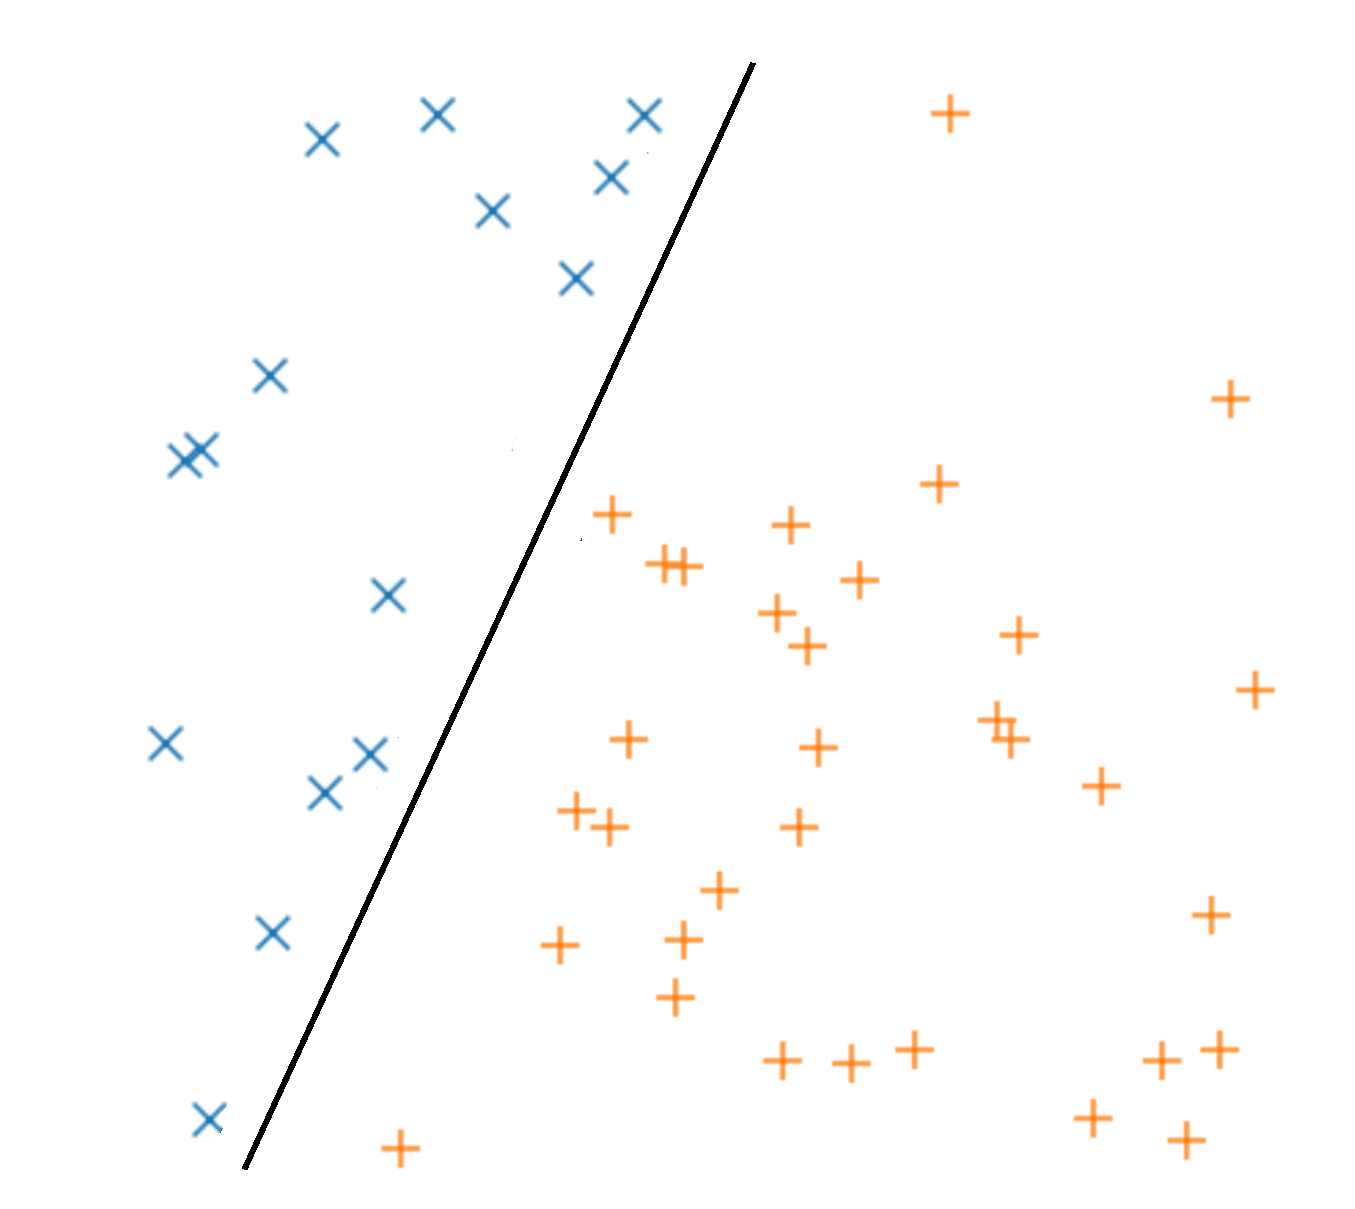
\includegraphics[width=0.35\textwidth]{Images/separabledroite.pdf}};		
			\node (label)[]  at([yshift = -5]ref.south) {Classifieur linéaire};
			%
			%
			\node (ref1) at([xshift =90]ref.east)
			{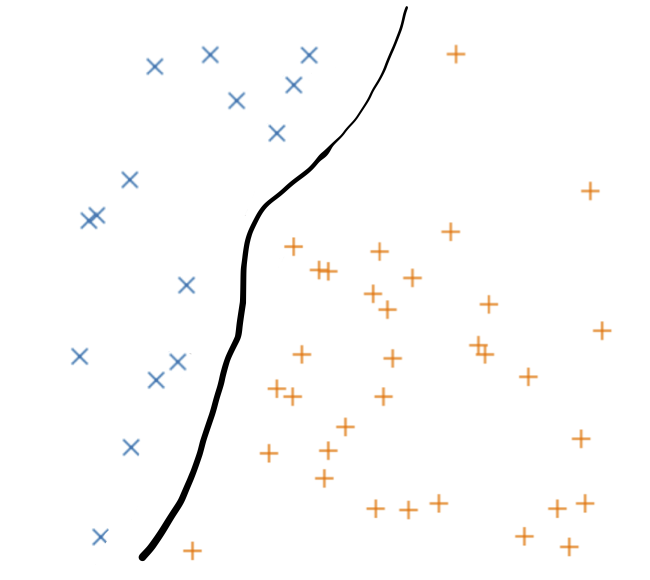
\includegraphics[width=0.35\textwidth]{Images/separablecourbe.png}};
			\node (label1)[]  at([yshift = -5]ref1.south) {Classifieur non linéaire};
			
		\end{tikzpicture}
		

	\end{center}
	
	\vspace*{2em}
	\bftitle{Classifieur linéaire} \\
	\textbf{Dans le cas de la classification binaire}, un classifieur linéaire va découper $\X$ en deux parties séparées par un hyperplan ( autrement dit une droite quand $d=2$) : d'un côté de l'hyperplan, les points auront l'étiquette $0$ et de l'autre, ils auront l'étiquette $1$. \\[0.5em] Autrement dit,\textbf{ la frontière de décision est un hyperplan}
	\note{dans le cas de la régression, on a une droite}
	\end{frame}
%------------------------------------------------------------------------------------------
%------------------------------------------------------------------------------------------
\begin{frame}{Classifieur linéaire - formulation}
		\begin{itemize}
		\item $\X = \bbR^d$, $d \geq 1$\\[1em]
	\end{itemize}
	
	On a vu qu'on cherchait le classifieur $\hat{f}^*$ qui minimise le risque empirique (pour une fonction de coût $\ell$ donnée) :
$\hat{f}^*= \text{{arg}}\,\min\limits_{f \in \F}\, \dfrac{1}{n} \sum_{i=1}^n \ell\left(y_i, f(x_i)\right)$\\[1em]
	
	Mais plutôt que de chercher $\hat{f}^*$ dans le plus grand ensemble $\F$ des fonctions mesurables, on restreint notre recherche : on cherche $\hat{f}^*$ dans un sous ensemble $\H \subset \F$ (biais inductif).  À quoi correspond  l'ensemble $\H$ des classifieurs linéaires ?\\[1em]
%	
%	En pratique, on cherche $\hat{f}^*$ dans un sous ensemble $\H \subset \F$ car pour\\\phantom{\bftitle{Remarque} \hsp}certaines raisons (nature du problème, éviter le surapprentissage)\\\phantom{\bftitle{Remarque} \hsp} on pense qu'il est préférable de restreindre notre recherche à $\H$.\\\phantom{\bftitle{Remarque} \hsp}Le choix de $\H$ représente donc une information a priori ; on appelle\\\phantom{\bftitle{Remarque} \hsp}cela un \textbf{biais inductif } 
	\pause
\begin{minipt}[0.1]{0.5}
	%\begin{center}
	\raisebox{1.5mm}{\bclampe \xspace} 
	
\end{minipt}
\begin{minipc}[0.89]{0.5}
Puisqu'un classifieur linéaire permet d'estimer l'étiquette d'un point en fonction de sa position par rapport à un hyperplan séparateur alors un classifieur linéaire va être \textit{composé de deux parties} :\\

\begin{enumerate}
	\item une partie qui permet de sélectionner/fixer un hyperplan\\[0.5em]
	\item une partie qui permet de savoir où un point $x \in \X$ se situe par rapport à cet hyperplan et donc d'estimer l'étiquette de $x$ 
\end{enumerate}
\end{minipc}
	
\end{frame}
%------------------------------------------------------------------------------------------
%------------------------------------------------------------------------------------------
%------------------------------------------------------------------------------------------
%------------------------------------------------------------------------------------------
\begin{frame}{Classifieur linéaire - formulation}
	\begin{enumerate}
	\item Partie qui permet de sélectionner/fixer un hyperplan : on considère l'ensemble des fonction affines de $\bbR^d$ dans $\bbR$
	
	$$ L_d = \left\{h_{\mathbf{w},b} : x \mapsto \langle \mathbf{w}, \mathbf{x}\rangle + b, \hsp \mathbf{w} \in \bbR^d, b \in \bbR\right\}$$
	
	À chaque fonction affine $h_{\mathbf{w},b}$ on peut associer l'hyperplan d'équation $\langle \mathbf{w}, \mathbf{x}\rangle + b = 0$. En classification, pour un point $x\in \X$, $h_{\mathbf{w},b}(x)$ donne de l'information sur la position de $x$ par rapport à cet hyperplan. \\[0.5em]
	
	\textcolor{MPTblue}{Remarque} \hsp quand $d=2$, la droite d'équation $\langle \mathbf{w}, \mathbf{x}\rangle + b = 0$ avec $\mathbf{w}=(w_1,w_2), \mathbf{x}=(x_1,x_2) \in \bbR^2$ correspond à la droite de pente $ -w_1/w2 $ et d'ordonnée à l'origine $-b/w_2$ \\[2em]
	

	\item Partie qui permet de savoir où un point $x \in \X$ se situe par rapport à cet hyperplan et donc d'estimer l'étiquette de $x$ : cette partie sera gérée par une fonction $\phi$\\[1em]
	
	
	\end{enumerate}
	
	
	Les classifieurs linéaires sont des fonctions qui s'écrivent comme la composée d'une fonction affine avec la une fonction $\phi$
	
	
	\note{faire exemple quand $d=2$ : retrouver la forme conventionnelle de la droite }
\end{frame}
%------------------------------------------------------------------------------------------
%------------------------------------------------------------------------------------------

\begin{frame}{Classifieur linéaire - formulation}
	

	
	
	\bftitle{Définition}
	%\vspace*{-0.2em}
	\begin{vblock}{}
		Les \bfblue{classifieurs linéaires} sont toutes les fonctions appartenant aux ensembles $\H_\phi$ , avec $\phi : \bbR \to \Y$,  définis par 
		% formés d'une famille de classes d'hypothèse : $$\H =\cup_{\phi} \, \H_\phi$$
		
		$$\H_\phi := \left\{\mathbf{x}\mapsto \phi  \ \circ \ h_{\mathbf{w},b}  (\mathbf{x}), \hsp  h_{\mathbf{w},b} \in L_d\right\}$$
		\vspace*{-1.5em}
		%et $\phi : \bbR \to \Y$
		%$\Phi = \{ \text{functions de } \bbR \text{ dans } \Y\}$
	\end{vblock}
	Les ensembles $\H_\phi$ sont appelées \textbf{des classes d'hypothèse}\\[2em]
	\pause

	\bftitle{Remarques} \\[.5em] 
\begin{itemize}
	\item La classe des classifieurs linéaires contient aussi bien des classifieurs  utilisés pour des problèmes de regréssion que des classifieurs utilisés pour des problèmes de classification (ou pour les deux, comme nous le verrons pour la régression logistique)\\[1em] 
	\item Souvent, le choix de la fonction $\phi$ considérée va dépendre du type de problème (classification ou régression) ainsi que de la fonction de coût $\ell$ considérée
\end{itemize}



\end{frame}
%------------------------------------------------------------------------------------------
%------------------------------------------------------------------------------------------


\begin{frame}{Classifieur linéaire - Optimisation}


On cherche donc $\hat{f}^*$ qui minimise le risque empirique lorsque, pour une fonction $\phi$ choisie adéquatement, on restreint notre recherche à $\H_\phi$ :

%\vspace*{-1em}
$$\hat{f}^*= \text{{arg}}\,\min\limits_{f \in \color{MPTred} \H_\phi}\, \color{black}  \dfrac{1}{n} \sum_{i=1}^n \ell\left(y_i, f(x_i)\right)$$\\[1em]
%\vspace*{-1em}

La fonction $\phi$ étant fixée, on se retrouve donc à chercher $ \left(\widehat{\mathbf{w}},\widehat{b}\right)$
qui minimise le risque empirique :
%un hyperplan,$\widehat{\mathbf{w}}$ (le vecteur orthogonal à l') et $\widehat{b}$ (l'ordonnée à l'origine) qui minimise le risque empirique suivant

\begin{equation} \left(\widehat{\mathbf{w}},\widehat{b}\right)= \text{{arg}}\,\min\limits_{\mathbf{w} \in \bbR^d \, b \in \bbR}\, \dfrac{1}{n}  \displaystyle \sum_{i=1}^n \ell\ \left(y_i, \phi\left( \langle {\mathbf{w}},x_i \rangle + b\right) \right)
	\label{eq:opti}
	\end{equation}

\vspace*{2em}

%	\bftitle{Remarques} \\[.5em] 
%	\begin{itemize}
%		\item La classe des classifieurs linéaires contient aussi bien des classifieurs  utilisés pour des problèmes de regréssion que des classifieurs utilisés pour des problèmes de classification (ou pour les deux, comme nous le verrons pour la régression logistique)\\[1em] 
%		\item Souvent, le choix de la fonction $\phi$ considérée va dépendre du type de problème (classification ou régression) ainsi que de la fonction de coût $\ell$ considérée
%	\end{itemize}


\end{frame}
%------------------------------------------------------------------------------------------
%------------------------------------------------------------------------------------------
\begin{frame}{Classifieur linéaire : pertinence ?}
Si on fait le choix de se restreindre à la famille des classifieurs linéaires $\H$ pour prédire l'étiquette d'un nouveau point $x \in \X$, c'est qu'on a de bonnes raisons de penser que ce type de classifieurs aura des chances d'avoir de bonnes performances. \\[0.5em]

En classification binaire \eg, c'est le cas lorsque les données observées semblent être plus ou moins linéairement séparables. Si les données sont loin d'être linéairement séparables, on préfèrera utiliser un classifieur non linéaire.\\

	\vspace*{0.5em}
	\begin{center}
	\begin{tikzpicture}
		\node(ref){\includegraphics[width=0.27\textwidth]{Images/separable.pdf}};		
		%\node (label)[]  at([yshift = -5]ref.south) {Classifieur linéaire};
		%
		%
		\node (ref1) at([xshift =70]ref.east)
		{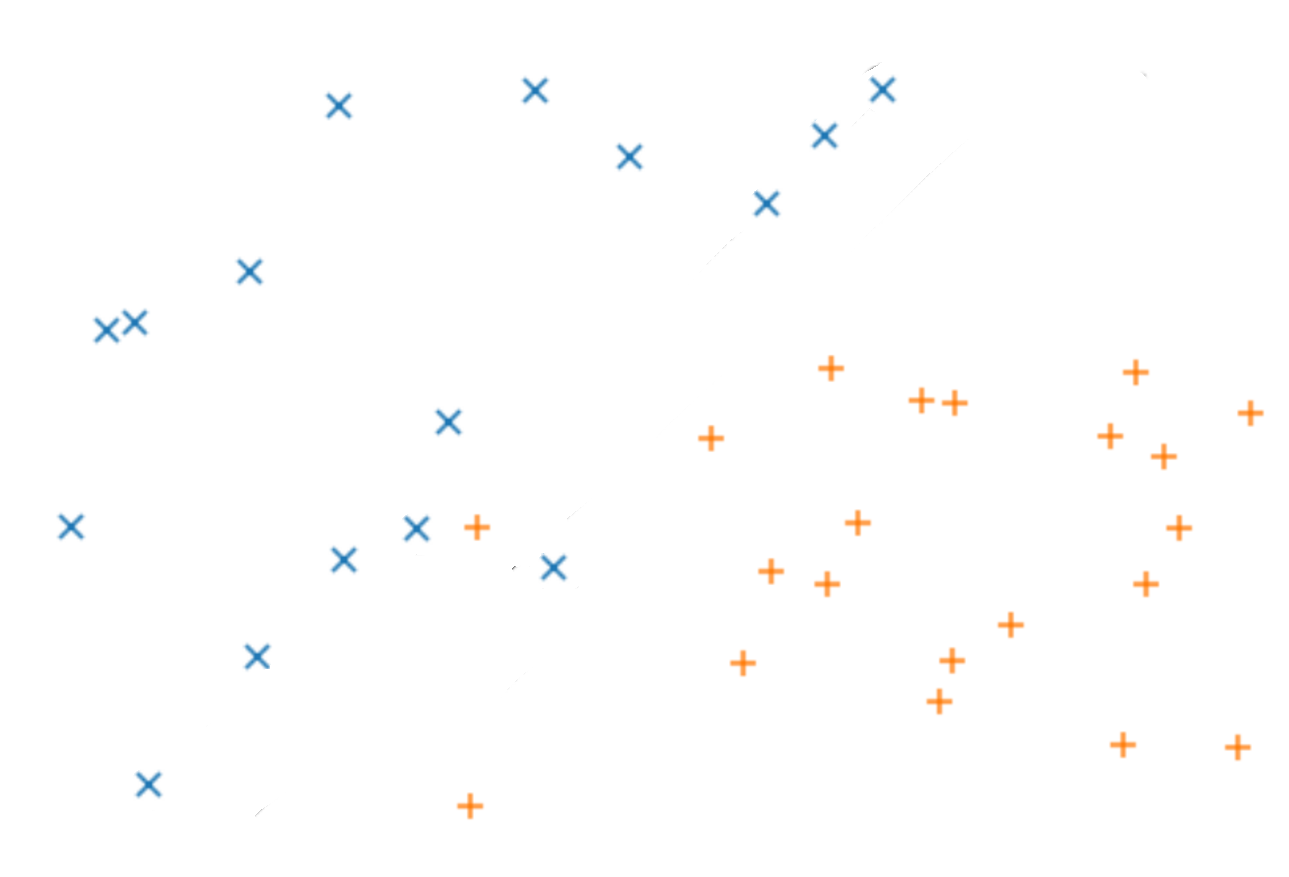
\includegraphics[width=0.27\textwidth]{Images/nonseparable.pdf}};
	%	\node (label1)[]  at([yshift = -5]ref1.south) {Classifieur non linéaire};
			\node (ref2) at([xshift =70]ref1.east)
		{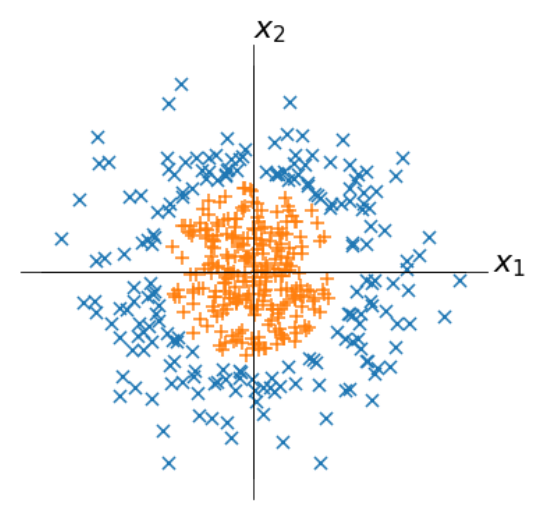
\includegraphics[width=0.27\textwidth]{Images/nonseparablecercle.png}};
		%
	\end{tikzpicture}
	
	
\end{center}

	\vspace*{0.5em}
	
		\begin{minipage}[c][2cm][t]{0.17\textwidth}
			\bftitle{Remarque} 
		\end{minipage}
		\begin{minipage}[c][2cm][t]{0.81\textwidth}
	En dimension 2, il est facile d'estimer si les données semblent plutôt linéairement séparables. Mais dès que la dimension augmente, c'est plus difficile ! C'est pourquoi il est important d'avoir un avis d'experts sur les données. 
		\end{minipage}
\end{frame}
%------------------------------------------------------------------------------------------
%------------------------------------------------------------------------------------------
\begin{frame}{Classifieurs linéaires et non-linéaires}
	
	Dans ce cours, nous avons vu ou verrons :\\[2em]
	
	\bftitle{Classifieurs linéaires} \\
	\begin{itemize}
		\item \only<1>{La régression logistique}\only<2>{\textbf{La régression logistique}}
		\item les SVM
	\end{itemize}
	
	\vspace*{3em}
	
		\bftitle{Classifieurs non linéaires} \\
	\begin{itemize}
		\item l'algorithme des KNN (régression et classification)
		\item Les arbres de décision (CART : régression et classification)
		\item les SVM à noyaux
	\end{itemize}
	\vspace*{3em}
	
	\note{dire quand c'est que classification ou quand c'est les deux : régression et classification}
\end{frame}
%------------------------------------------------------------------------------------------
%------------------------------------------------------------------------------------------


%------------------------------------------------------------------------------------------
%------------------------------------------------------------------------------------------


\subsection{Classifieurs Linéaires\\[0.5em] --\\[0.5em]  La régression logistique}

%------------------------------------------------------------------------------------------
\begin{frame}{Préliminaires : classifieur des demi-espaces}
	\vspace*{-0.5em}
	Sans perte de généralité, on suppose que $\Y = \{-1,1\}$\\[1em]
	
	Avant de voir  la régression logistique, on peut s'intéresser à un premier classifieur linéaire : \textbf{le classifieur des demi-espaces}
	\vspace*{25em}
\end{frame}


%------------------------------------------------------------------------------------------
\begin{frame}{}
	
\end{frame}
%%------------------------------------------------------------------------------------------
%------------------------------------------------------------------------------------------
\begin{frame}{}
	
\end{frame}
%%------------------------------------------------------------------------------------------
%------------------------------------------------------------------------------------------
\begin{frame}{}
	
\end{frame}
%%------------------------------------------------------------------------------------------
%------------------------------------------------------------------------------------------
\begin{frame}{}
	
\end{frame}
%%------------------------------------------------------------------------------------------
%------------------------------------------------------------------------------------------
\begin{frame}{}
	
\end{frame}
%%------------------------------------------------------------------------------------------
%------------------------------------------------------------------------------------------
\begin{frame}{}
	
\end{frame}
%%------------------------------------------------------------------------------------------
%------------------------------------------------------------------------------------------
\begin{frame}{}
	
\end{frame}
%%------------------------------------------------------------------------------------------
%------------------------------------------------------------------------------------------
\begin{frame}{}
	
\end{frame}
%%------------------------------------------------------------------------------------------
%------------------------------------------------------------------------------------------
\begin{frame}{}

\end{frame}
%%------------------------------------------------------------------------------------------
%------------------------------------------------------------------------------------------
\begin{frame}{}
%confiance en la prédiction : proche ou pas de la droite
\end{frame}


%%------------------------------------------------------------------------------------------




\begin{frame}{La régression logistique}
	\begin{itemize}
		\item $\Y = \{-1,1\}$\\[-1em]
	\end{itemize}
	\begin{minipc}[0.1]{0.2}
		%\begin{center}
		\raisebox{1.5mm}{\bclampe \xspace} 
		
	\end{minipc}
	\begin{minipc}[0.89]{0.2}
		Au lieu de prendre $\phi (z) =  sign(z) \in \{-1,1\}$, on considère la \textbf{fonction sigmoïde} qui retourne un nombre dans $[0,1]$ afin de nuancer la confiance en la labellisation effectuée :
		
	
	\end{minipc}
	
		$$ \phi_{sig}(z) = \dfrac{1}{1+ \exp(-z)}\hsp\hsp\hsp z \in \bbR$$
	
	\vspace*{0.5em}
	En effet, $ \phi_{sig}$ est croissante et $\lim\limits_{z\to - \infty} \phi(z)= \todo{\phantom{\,\,\,}}{0\,\,}$, $\lim\limits_{z\to  \infty} \phi(z)= \todo{\phantom{\,\,\,}}{1\,\,}$
	\vspace*{10em}

\end{frame}

%%------------------------------------------------------------------------------------------
%%------------------------------------------------------------------------------------------

\begin{frame}{}
	Soit $x\in \X$ et l'hyperplan $H$ d'équation $\langle {\mathbf{w}},x\rangle + b=0$  \\[2em]
	
	\begin{itemize}
		\item $z=\langle {\mathbf{w}},x\rangle + b > 0$ et très grand :  \\[1em]
	
	\begin{itemize}
		\item[] $x$ est \todo{\phantom{au-dessus}}{au-dessus} et \todo{\phantom{loin}}{loin} de $H$\\[0.5em]
		\item[] $\phi_{sig}(z) $ proche de \todo{\phantom{$1$}}{$1$} \\[2em]
	\end{itemize}
	
	\item  $z=\langle {\mathbf{w}},x\rangle + b < 0$ et $|z|$ très grand : \\[1em]
	
	\begin{itemize}
		\item[] $x$ est \todo{\phantom{en dessous}}{en dessous} et \todo{\phantom{loin}}{loin} de $H$\\[0.5em]
		\item[]  $\phi_{sig}(z) $ proche de \todo{\phantom{$0$}}{$0$} \\[2em]
	\end{itemize}
	
\item  $z=\langle {\mathbf{w}},x\rangle + b $  proche de 0 :  \\[1em]
	
	\begin{itemize}
		\item[] $x$ est \todo{\phantom{proche}}{proche} de $H$ :  \todo{\phantom{en dessous si $|z|<0$, au-dessus si $|z|>0$}}{en dessous si $|z|<0$, au-dessus si $|z|>0$}\\[0.5em]
		\item[] $\phi_{sig}(z) $ proche de  \todo{\phantom{$1/2$}}{$1/2$}  \\[1.5em]
	\end{itemize}
	\end{itemize}
	
	
	
\end{frame}


%%------------------------------------------------------------------------------------------
%%------------------------------------------------------------------------------------------

\begin{frame}{}
	Puisque $\phi_{sig} (z) =  sign(z) \in [0,1]$ : le classifieur renvoie donc un nombre dans $[0,1]$\\[0.5em]
	 Quelle étiquette $\hat{y}$ prédire pour une observation $x$, \ie quelle règle de décision adopter ?
	
	
	
	\vspace{5em}
	
L'étiquette donnée est la même que celle donnée par le classifieur des demi-espaces sauf qu'ici, la fonction sigmoïde $\phi_{sig}$ permet de nuancer notre estimation : \\[1em]
\begin{itemize}
	\item si $x$ est proche de l'hyperplan, $\phi_{sig} (\langle\mathbf{w},x\rangle + b)$  est proche de $1/2$ : \\[4em]
	
	\item si $x$ est loin de l'hyperplan, $\phi_{sig} (\langle\mathbf{w},x\rangle + b)$  est proche de $0$ ou $1$ : \\[4em]
\end{itemize}
	\bfblue{Remarque} \hsp $\phi_{sig} (\langle\mathbf{w},x\rangle + b)$ peut-être interprétée comme la probabilité pour que l'étiquette de $x$ soit égale à $1$
\end{frame}

%%------------------------------------------------------------------------------------------
%%------------------------------------------------------------------------------------------

\begin{frame}{}
	Maintenant que $\phi = \phi_{sig}$ a été choisie, quelle fonction de coût $\ell$ adopter ?\\[2em]
	
	\bfblue{Remarque} \hsp La fonction de coût $\ell$ va nous permettre de trouver les paramètres $(\widehat{\mathbf{w}},\widehat{b})$ qui vérifient l'équation \eqref{eq:opti}\\[1em]
	
	Pour $(x,y) \in \X \times \Y$,  \\
	\begin{itemize}
		\item \phantom{a}\\[3em]
		\item  \phantom{a}\\[3em]
			\item  \phantom{a}\\[4em]
	\end{itemize}
	
On souhaite donc que la pénalisation ne dépende plus uniquement de la position de $x$ par rapport à l'hyperplan mais également de sa distance à l'hyperplan\\[1em]
%		\begin{minipc}[0.12]{0.15}
%		%\begin{center}
%		\raisebox{1.5mm}{\bclampe \xspace} 
%	\end{minipc}
%	\begin{minipc}[0.87]{0.15}
%		On souhaite prendre $\ell$ qui croît de manière monotone par rapport à 
%	\end{minipc}
	
\end{frame}

%%------------------------------------------------------------------------------------------
%%------------------------------------------------------------------------------------------

\begin{frame}
	Pour déterminer quelle fonction $\ell$ choisir, détaillons deux cas :\\[1em]
	
	\begin{itemize}
		\item Cas $y=1$\\[10em]
		
			\item Cas $y=-1$\\[10em]
	\end{itemize}
	On veut donc une fonction $\ell$ qui augmente quand $\displaystyle 1+ \exp\left(-y\left(\langle w,x\rangle +b\right)\right)$ augmente : on va considérer la fonction $\log$
\end{frame}

%%------------------------------------------------------------------------------------------
%%------------------------------------------------------------------------------------------
\begin{frame}
	Pour déterminer quelle fonction $\ell$ choisir, détaillons deux cas :\\[1em]
	
	\begin{itemize}
		\item Cas $y=1$\\[10em]
		
		\item Cas $y=-1$\\[9em]
	\end{itemize}
	On veut donc une fonction $\ell$ qui augmente quand $\displaystyle 1+ \exp\left(-y\left(\langle w,x\rangle +b\right)\right)$ augmente : on va considérer la fonction $\log$
\end{frame}

%%------------------------------------------------------------------------------------------
%%------------------------------------------------------------------------------------------


\begin{frame}
Quelle allure à la fonction $z =\langle w,x\rangle +b \mapsto \log\left(1+ \exp\left(-yz\right)\right)$ ?\\[1em]
\begin{itemize}
	\item Cas $y=1$   \\[11em]
	
	\item Cas $y=-1$\\[11em]
\end{itemize}

\end{frame}
%%------------------------------------------------------------------------------------------
%%------------------------------------------------------------------------------------------

\begin{frame}
À paritr des données d'apprentissage $(x_1,y_1), \dots, (x_n, y_n) \in \X \times \Y$, on cherche donc $ \left(\widehat{\mathbf{w}},\widehat{b}\right)$ tels que\\[1.5em]

%un hyperplan,$\widehat{\mathbf{w}}$ (le vecteur orthogonal à l') et $\widehat{b}$ (l'ordonnée à l'origine) qui minimise le risque empirique suivant

$$\begin{array}{lll}
	 \left(\widehat{\mathbf{w}},\widehat{b}\right)&=& 
	 %\text{{arg}}\,\min\limits_{\mathbf{w} \in \bbR^d \, b \in \bbR}\, \dfrac{1}{n}  \displaystyle \sum_{i=1}^n \ell\ \left(y_i, \phi_{sig}\left( \langle {\mathbf{w}},x_i \rangle + b\right) \right)\\[2.5em]
	 %	&=& 
	 	\text{{arg}}\,\min\limits_{\mathbf{w} \in \bbR^d \, b \in \bbR}\, \dfrac{1}{n}  \displaystyle \sum_{i=1}^n  \log\left(1+ \exp\left(-y_i\left[\langle w,x_i\rangle +b\right]\right)\right)
\end{array}$$

\vspace{2em}

\bfblue{Remarque} \hsp Les paramètres $\widehat{\mathbf{w}}$ et $\widehat{b}$ de l'hyperplan optimal dépendent des données d'apprentissage $(x_1,y_1), \dots, (x_n, y_n)$)\\[1em]

Pour une nouvelle observation $x$, on estime $\hat{y} =1$ si  $\phi_{sig}\left( \langle \widehat{\mathbf{w}},x \rangle + \widehat{b}\right) \geq 0.5$, $\hat{y} =0$ sinon \\[1em]

De manière plus générale, on peut également décider que $\hat{y} =1$ si  $\phi_{sig}\left( \langle \widehat{\mathbf{w}},x \rangle + \widehat{b}\right) \geq \alpha$, avec $\alpha \in ]0,1[$. Le seuil $\alpha$ représente alors le niveau de confiance minimal qu'on est prêt à accepter pour décider que $\hat{y} =1$. Pour \eg $\alpha < 0.5$, cela a du sens lorsque\\[4em]

\end{frame}
%%------------------------------------------------------------------------------------------
%%------------------------------------------------------------------------------------------


\begin{frame}
Quelle différence entre le classifieur des demi-espaces et celui de la régression linéaire ?\\[24em]
\end{frame}

%%------------------------------------------------------------------------------------------
%%------------------------------------------------------------------------------------------


\begin{frame}{Évaluer un modèle avec l'AUC}
Une fois que les paramètres $({\mathbf{w}}, {b})$ d'un modèle de régression logistique ont été ajustés, on peut regarder les performances de ce modèle (en terme de classification) grâce aux métriques vues précédemment (accuracy, sensibilité, etc)\\[1em]

	\begin{minipc}[0.12]{0.15}
	%\begin{center}
	\raisebox{1.5mm}{\bclampe \xspace} 
\end{minipc}
\begin{minipc}[0.87]{0.15}
	On cherche à regarder comment évoluent les performances du modèle lorsqu'on change le niveau de confiance $\alpha$ qu'on est prêt à accepter pour décider que $\hat{y}=1$
\end{minipc}

\vspace*{16em}

\end{frame}

%%------------------------------------------------------------------------------------------
%%------------------------------------------------------------------------------------------
\begin{frame}
	
\end{frame}
%%------------------------------------------------------------------------------------------
%%------------------------------------------------------------------------------------------

\begin{frame}
	
\end{frame}
%%------------------------------------------------------------------------------------------
%%------------------------------------------------------------------------------------------

\begin{frame}
	\begin{itemize}
		\item Cas du classifieur parfait \\[24em]
	\end{itemize}
	
	
\end{frame}
%%------------------------------------------------------------------------------------------
%%------------------------------------------------------------------------------------------


\begin{frame}
		\begin{itemize}
		\item 	Cas du classifieur aléatoire \\[24em]
	\end{itemize}
\end{frame}
	
	%%------------------------------------------------------------------------------------------
	%%------------------------------------------------------------------------------------------
	
	\begin{frame}
\bftitle{Exercice} \hsp \\[24em]
		
	\end{frame}
	
	%%------------------------------------------------------------------------------------------
	%%------------------------------------------------------------------------------------------
	
	
	
	\begin{frame}
La courbe ROC peut nous aider à choisir le seuil $\alpha$ à considérer \\[24em]
		
	\end{frame}
	


%%------------------------------------------------------------------------------------------
%%------------------------------------------------------------------------------------------

\begin{frame}
	L'AUC (calculée sur l'échantilllon de validation) peut servir à choisir entre différents modèles \\[24em]
	
\end{frame}


%%------------------------------------------------------------------------------------------
%%------------------------------------------------------------------------------------------



\begin{frame}{La régression logistique multiclasse}
\begin{itemize}
	\item $\Y=\{1,\dots, C\}$\\[1em]
\end{itemize}
	
Plusieurs stratégies possibles\\[1em]

\vspace*{22em}

%\begin{enumerate}
%	\item 
%\end{enumerate}
	
	
\end{frame}

%%------------------------------------------------------------------------------------------
%%------------------------------------------------------------------------------------------


%\begin{frame}{}
%	
%Pour une fonction $\phi : \bbR \to \Y$ choisie adéquatement, on cherche $\widehat{\mathbf{w}}$ et $\widehat{b}$  tels que
%
%$$ \left(\widehat{\mathbf{w}},\widehat{b}\right)= \text{{arg}}\,\min\limits_{\mathbf{w} \in \bbR^d \, b \in \bbR}\, \dfrac{1}{n}  \displaystyle \sum_{i=1}^n \ell\ \left(y_i, \phi\left( \langle {\mathbf{w}},x_i \rangle + b\right) \right)$$
%
%avec $\H_\phi := \left\{\mathbf{x}\mapsto \phi  \ \circ \ h_{\mathbf{w},b}  (\mathbf{x}), \hsp  h_{\mathbf{w},b} \in L_d\right\}$
%	
%	\begin{center}
%		La régression logistique consiste à résoudre le problème de minimisation lorsque $\ell$ est le coût 
%	\end{center}
%
%\end{frame}
%%------------------------------------------------------------------------------------------
%
%%\subsection{Classifieurs Linéaires\\[0.5em] --\\[0.5em]  Le coût quadratique}
%%
%%\subsection{Classifieurs Linéaires\\[0.5em] --\\[0.5em]  Le coût logistique}
%
%\subsection{Classifieurs Linéaires\\[0.5em] --\\[0.5em]  Évaluer un modèle avec l'AUC}
%
%\subsection{Classifieurs Linéaires\\[0.5em] --\\[0.5em]  Classification Multiclasse}
%
%
%	



\begin{frame}{Références}
	\begin{thebibliography}{2}
			\vspace{-1.8em}
			
	%	\bibitem{1} L.~Bel, J.N.~Bacro and C.~Lantuéjoul, \textcolor{black}{Assessing extremal dependence of environmental spatial fields,} \emph{Environmetrics}, 19(2):163-182, 2008
		
		\bibitem{pouet} C.A.~Azencot \textcolor{black}{{\href{http://cazencott.info/dotclear/public/lectures/IntroML_Azencott.pdf}{Introduction au Machine Learning}}}, \emph{Dunod},\\ ISBN : 978-2-10-084143-1\\[2em]
		
	%	\bibitem{CNP2006} D.~Cooley, P.~Naveau and P.~Poncet \textcolor{black}{Variograms for spatial max-stable random fields}, pages 370-390, \emph{Springer New-York}, 2006
		
		\bibitem{2} S.~Shalev-Shwartz and S.~Ben-David, \textcolor{black}{Understanding Machine Learning: From Theory to Algorithms,} \emph{Cambridge University Press}, DOI : 10.1017/CBO9781107298019, 2014\\[2em]
		%
	%	\bibitem{3} C.~Dombry, S.~Engelke, M.~Oesting (2016) \textcolor{black}{Exact simulation of max-stable processes}, \textit{Biometrika} 103(2):303–317
		
		\bibitem{E} T.~Hastie, R.~Tibshirani, and J.~Friedman. \textcolor{black}{The Elements of Statistical Learning}, \emph{Springer New York}, DOI : 10.1007/978-0-387-84858-7, 2009
		
		
		%
		%	\bibitem{4} R.A.~Fisher and L.H.C.~Tippett, \textcolor{black}{Limiting forms of the frequency distribution of the largest or smallest member of a sample,} \emph{Mathematical Proceedings of the Cambridge Philosophical Society}, 24(2):180-190, 1928\\[0.3em]
		%	
	\end{thebibliography}
	
\end{frame}
\end{document}
